\documentclass{article}
\setlength{\parskip}{5pt} % esp. entre parrafos
\setlength{\parindent}{0pt} % esp. al inicio de un parrafo
\usepackage{amsmath} % mates
\usepackage{listings}
\usepackage[sort&compress,numbers]{natbib} % referencias
\usepackage{url} % que las URLs se vean lindos
\usepackage[top=25mm,left=20mm,right=20mm,bottom=25mm]{geometry} % margenes
\usepackage{hyperref} % ligas de URLs
\usepackage{graphicx} % poner figuras
\usepackage[spanish]{babel} % otros idiomas
\usepackage{textcomp}
\usepackage{pgfplots} % crear graficas
\pgfplotsset{width=9cm,compat=1.7}
\title{"P11" Frentes de Pareto} %Título
\author{NESTOR}
\date{Mayo 2022}

\begin{document} % inicia contenido

\maketitle % cabecera


 

\section{Objetivo}
El objetivo se trata de en optimización multicriterio, a un mismo conjunto de variables ocupa asignarse valores de tal forma que se optimizen dos o más funciones objetivo, que pueden contradecir una a otra — una mejora en una puede corresponder en una empeora en otra. Además hay que respetar potenciales restricciones, si es que haya.

Para estudiar este problema, vamos a primero implementar un generador de polinomios aleatorios. Estos polinomios los utilizaremos como funciones objetivo. Vamos a permitir solamente una variable por término y un término por grado por variable \cite{elisa1}.

\section{Desarrollo}\label{des}
De acuerdo con el desarrollo en el código de la  \href{https://github.com/satuelisa/Simulation/blob/master/ParetoFronts/poligen.py}{codificación} implementado por E. Schaeffer y todas las instrucciones se encuentran en el  \href{https://github.com/NestorZeus/SIMULACION-COMPUTACIONAL-DE-NANOMATERIALES/tree/main/P11}{repositorio} de N. Rodríguez en GitHub.\\

Para comenzar se implementa una solución aleatoria para polinomios que se generan al azar, con esto se crea la solución de polinomios y evaluación. A continuación se ejecuta el siguiente código:

\begin{lstlisting}
import numpy as np
from scipy import stats
import pandas as pd
from itertools import compress
from random import randint, random
import matplotlib.pyplot as plt

def poli(maxdeg, varcount, termcount):
    f = []
    for t in range(termcount):
        var = randint(0, varcount - 1)
        deg = randint(1, maxdeg)
        f.append({'var': var, 'coef': random(), 'deg': deg})
    return pd.DataFrame(f)
 
def domin_by(target, challenger):
    if np.any(challenger < target):
        return False
    return np.any(challenger > target)
 
vc = 4
md = 3
tc = 5
#k = 2 

replicas= 30
CV=[]
for k in range(2,6):
    rep=[]
    for r in range(replicas):
        obj = [poli(md, vc, tc) for i in range(k)]
        minim = np.random.rand(k) > 0.8
        n = 100
        sol = np.random.rand(n, vc)
        val = np.zeros((n, k))
        for i in range(n): 
            for j in range(k):
                val[i, j] = evaluate(obj[j], sol[i])
        sign = [1 + -2 * m for m in minim]
        dom = []
        for i in range(n):
            d = [domin_by(sign * val[i], sign * val[j]) for j in range(n)]
            dom.append(sum(d)) 
        frente = val[[d == 0 for d in dom], :]
        rep.append((len(frente)*100)/n)
    CV.append(rep)
fig, ax = plt.subplots(nrows = 1, ncols = 1, figsize=(4, 10))
plt.ylabel('Porcentaje (%) solución de pareto')
parts = ax.violinplot(CV, showmeans=False, showmedians=False, showextrema=False)
for p in parts['bodies']:
    p.set_facecolor('grey')
    p.set_edgecolor('green')
    p.set_alpha(1)
c='blue'
plt.xlabel('Función')
plt.savefig('p11p_violin.png', bbox_inches = 'tight')
plt.close()
print(result)
\end{lstlisting}


\section{Resultados}
El rango de las soluciones de porcentaje no dominada se empieza a distribuir los porcentajes de las distribuciones de los porcentajes.


\begin{figure_1}
    \centering
    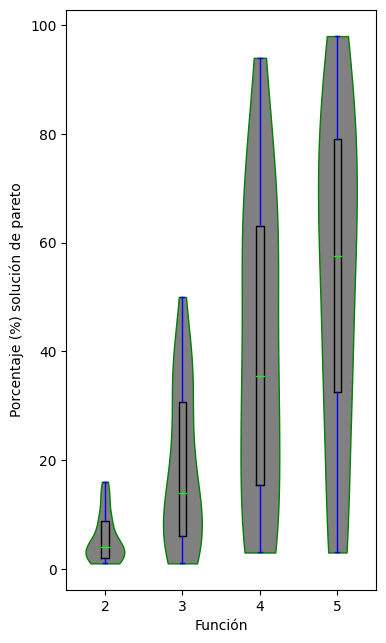
\includegraphics[width=90mm]{p11p_violin.png}
    \caption{Figura 1: Diagrama violín distribucion de porcentaje}
    \label{figure_1}

\section{Conclusiones}

Es complicado saber hayar una solución eficiente de una menor cantidad de funciones esto debido a que aumenta el rango de porcentajes de soluciones no encontradas.


\bibliography{simulacion}
\bibliographystyle{plainnat}
\end{document}
